%------------------------------------------------------------------------------%

\usepackage{calculo_varias_variaveis-1}

\title{Curvas Paramétricas}

%------------------------------------------------------------------------------%
\begin{document}

\addtitle

%------------------------------------------------------------------------------%
\section{Introdução}

\framedgraphic{Trajetória}{trajeto_maps}{}

%------------------------------------------------------------------------------%
\begin{frame}{Curvas Paramétricas}
  Funções de $\R$ em $\R^n$
  \[
    (x, y) = \big( f(t), g(t) \big)
  \]
  ou
  \[
  \left[\begin{array}{>{\,}c<{\,}}
    x \\[1mm]
    y
  \end{array}\right]
  =
  \left[\begin{array}{>{\,}c<{\,}}
    f(t) \\[1mm]
    g(t)
  \end{array}\right]
  \]

  \pause
  \vspace{\baselineskip}
  Podemos pensar na variável como o tempo e a curva como uma trajetória
\end{frame}

%------------------------------------------------------------------------------%
\section{Curvas Paramétricas}

%------------------------------------------------------------------------------%
\begin{frame}{Definição em 2D}
  Se $x$ e $y$ são dados como funções
  \[
    x = f(t)
    \qquad
    y = g(t)
  \]
  sobre um intervalo $I$ de valores de $t$,
  \pause
  então o conjunto de pontos
  \[
    (x, y) = \big( f(t), g(t)\big)
  \]
  \pause
  forma uma \emph{curva paramétrica} em $\R^2$

  \pause
  As equações são as \emph{equações paramétricas} da curva
\end{frame}

%------------------------------------------------------------------------------%
\begin{frame}{Definição em 3D}
  Se $x$, $y$ e $z$ são dados como funções
  \[
    x = f(t)
    \qquad
    y = g(t)
    \qquad
    z = h(t)
  \]
  sobre um intervalo $I$ de valores de $t$,
  então o conjunto de pontos
  \[
    (x, y, z) = \big( f(t), g(t), h(t) \big)
  \]
  forma uma \emph{curva paramétrica} em $\R^3$
\end{frame}

%------------------------------------------------------------------------------%
\begin{frame}{Definição Geral}
  Se $x_i$, $i=1, \dots, n$ são as coordenadas no espaço $\R^n$
  \[
    x_i = f_i(t)
  \]
  sobre um intervalo $I$ de valores de $t$,
  então o conjunto de pontos
  \[
    (x_1, x_2, \dots, x_n) = \big( f_1(t), f_2(t), \dots, f_n(t)\big)
  \]
  forma uma \emph{curva paramétrica} em $\R^n$
\end{frame}

%------------------------------------------------------------------------------%
\begin{frame}{Nomenclatura}
  \emph{$t$} \quad é o parâmetro da curva

  \pause
  \emph{$I$} \quad intervalo do parâmetro

  \pause
  \vspace{\baselineskip}
  Se $I$ é um intervalo fechado \emph{\(a\leq t \leq b\)}
  \pause
  \begin{description}[<+->]
    \item[\(\big(f(a), g(a)\big)\)] é o ponto inicial
    \item[\(\big(f(b), g(b)\big)\)] é o ponto final
  \end{description}
\end{frame}

%------------------------------------------------------------------------------%
\begin{frame}{Notações}
  \[
    (x, y)
    = \big(x(t), y(t)\big)
    = \big(f(t), g(t)\big)
  \]

  \pause
  \[
      \begin{pmatrix}  x    \\ y    \end{pmatrix}
    = \begin{pmatrix}  x(t) \\ y(t) \end{pmatrix}
    = \begin{pmatrix}  f(t) \\ g(t) \end{pmatrix}
  \]

  \pause
  \[
    (x_1, x_2, \dots, x_n) = \big( f_1(t), f_2(t), \dots, f_n(t)\big)
  \]
\end{frame}

%------------------------------------------------------------------------------%
\section{Exemplos}

% 01
%------------------------------------------------------------------------------%
\addtocounter{exemplo}{1}
\begin{frame}{Exemplo \theexemplo}
  Trace a curva definida pelas equações paramétricas
  \[
    x = t^2       \qquad
    y = t + 1     \qquad
    -\infty < t < \infty
  \]
\end{frame}

%------------------------------------------------------------------------------%
\begin{frame}{Exemplo \theexemplo}
\begin{columns}
\column{0.3\linewidth}
  Note que

  \pause
  \vspace{\baselineskip}
  $y$ varia com $t$ e

  \pause
  \vspace{\baselineskip}
  $x$ varia com $t^2$

\column{0.5\linewidth}
  \pause
  Calculando alguns pontos
  \[
    \begin{array}{r<{\qquad}r<{\quad}r}
      \hline
      t  & x & y  \\ \hline
      -3 & 9 & -2 \\
      -2 & 4 & -1 \\
      -1 & 1 & 0  \\
      0  & 0 & 1  \\
      1  & 1 & 2  \\
      2  & 4 & 3  \\
      3  & 9 & 4  \\ \hline
    \end{array}
  \]
\end{columns}
\end{frame}

%------------------------------------------------------------------------------%
\begin{frame}{Exemplo \theexemplo}
  \centering
  
\includegraphics[height=0.6\textheight]{exemplo_curvas_1}
\end{frame}

% 02
%------------------------------------------------------------------------------%
\addtocounter{exemplo}{1}
\begin{frame}{Exemplo \theexemplo}
  Identifique geometricamente a curva do Exemplo 1 eliminando o parâmetro $t$
  \[
    x = t^2        \qquad
    y = t + 1      \qquad
    -\infty < t < \infty
  \]

  \pause
  Transformar a curva paramétrica em $t$ em uma equação envolvendo $x$ e $y$
\end{frame}

%------------------------------------------------------------------------------%
\begin{frame}{Exemplo \theexemplo}
\begin{columns}
\column{0.3\linewidth}
  \onslide<+->{Eliminar $t$ em
  \begin{align*}
    x & = t^2   \\
    y & = t + 1
  \end{align*}}

\column{0.3\linewidth}
  \begin{align*}
    \onslide<+->{y & = t + 1 \\}
    \onslide<+->{t & = y - 1}
  \end{align*}

\column{0.3\linewidth}
  \begin{align*}
    \onslide<+->{x & = t^2} \\
    \onslide<+->{  & = (y - 1)^2} \\
    \onslide<+->{  & = y^2 - 2y + 1}
  \end{align*}
\end{columns}
\end{frame}

% 03
%------------------------------------------------------------------------------%
\addtocounter{exemplo}{1}
\begin{frame}{Exemplo \theexemplo}
  Determine se os pontos \((2, 3)\) e \((4, -1)\) pertencem a curva paramétrica
  \[
    x = t^2       \qquad
    y = t + 1     \qquad
    -\infty < t < \infty
  \]
\end{frame}


%------------------------------------------------------------------------------%
\begin{frame}{Exemplo \theexemplo}
\begin{columns}[t]
\column{0.4\linewidth}
  \onslide<+->{Testando o ponto \((2, 3)\)}
  \begin{align*}
    \onslide<+->{y & = 3} \\[2mm]
    \onslide<+->{t & + 1 = 3}         \\[2mm]
    \onslide<+->{t & = 3 -1}
    \onslide<+->{ = 2}      \\[2mm]
    \onslide<+->{x & = t^2}
    \onslide<+->{ = 2^2}
    \onslide<+->{ = 4}
    \onslide<+->{\neq 2}
  \end{align*}
  \onslide<+->{O ponto não pertence a curva}

\column{0.4\linewidth}
\onslide<+->{Testando o ponto \((4, -1)\)}
\begin{align*}
  \onslide<+->{y & = -1}               \\[2mm]
  \onslide<+->{t & + 1 = -1}           \\[2mm]
  \onslide<+->{t & = -1 -1}
  \onslide<+->{ = -2}       \\[2mm]
  \onslide<+->{x & = t^2}
  \onslide<+->{ = (-2)^2}
  \onslide<+->{ = 4}
\end{align*}
\onslide<+->{O ponto pertence a curva}
\end{columns}
\end{frame}

% 04
%------------------------------------------------------------------------------%
\addtocounter{exemplo}{1}
\begin{frame}{Exemplo \theexemplo}
  Represente graficamente a curva paramétrica
  \[
    x = \cos(t)         \qquad
    y = \sin(t)         \qquad
    0 \leq t \leq 2\pi
  \]
\end{frame}

%------------------------------------------------------------------------------%
\begin{frame}{Exemplo \theexemplo}
  Sabemos que essa é a parametrização do circulo trigonométrico

  \pause
  Calculando alguns pontos
  \[
  \renewcommand*{\arraystretch}{1.7}
  \begin{array}{c<{\quad}r<{\quad}r}
    \hline
    t               & x  & y  \\ \hline
    0               & 1  & 0  \\
    \dfrac{\pi}{2}  & 0  & 1  \\
    \pi             & -1 & 0  \\
    \dfrac{3\pi}{2} & 0  & -1 \\
    2\pi            & 1  & 0  \\ \hline
  \end{array}
  \]
\end{frame}

%------------------------------------------------------------------------------%
\begin{frame}{Exemplo \theexemplo}
  \centering
  
\includegraphics[height=0.6\textheight]{exemplo_curvas_3}
\end{frame}

%------------------------------------------------------------------------------%
\addtocounter{exemplo}{1}
\begin{frame}{Exemplo \theexemplo}
  Esboce a trajetória definida pela curva paramétrica
  \[
  \begin{cases}
    x = t \cos(t\pi) \\
    y = t \sin(t\pi)
  \end{cases}
  \]
  \(0\leq t\)
\end{frame}

%------------------------------------------------------------------------------%
\begin{frame}{Exemplo \theexemplo}
  Similar a parametrização do circulo trigonométrico

  \pause
  \[
  \renewcommand*{\arraystretch}{1.9}
  \begin{array}{c<{\quad}c<{\quad}c<{\quad}c<{\quad}c<{\quad}c}
    \hline
    t            & t\pi            & \cos(t\pi) & \sin(t\pi) & x  & y             \\ \hline
    0            & 0               & 1          & 0          & 0  & 0             \\
    \dfrac{1}{2} & \dfrac{\pi}{2}  & 0          & 1          & 0  & \dfrac{1}{2}  \\
    1            & \pi             & -1         & 0          & -1 & 0             \\
    \dfrac{3}{2} & \dfrac{3\pi}{2} & 0          & -1         & 0  & -\dfrac{3}{2} \\
    2            & 2\pi            & 1          & 0          & 2  & 0             \\ \hline
  \end{array}
  \]
\end{frame}

%------------------------------------------------------------------------------%
\begin{frame}{Exemplo \theexemplo}
  \centering
  

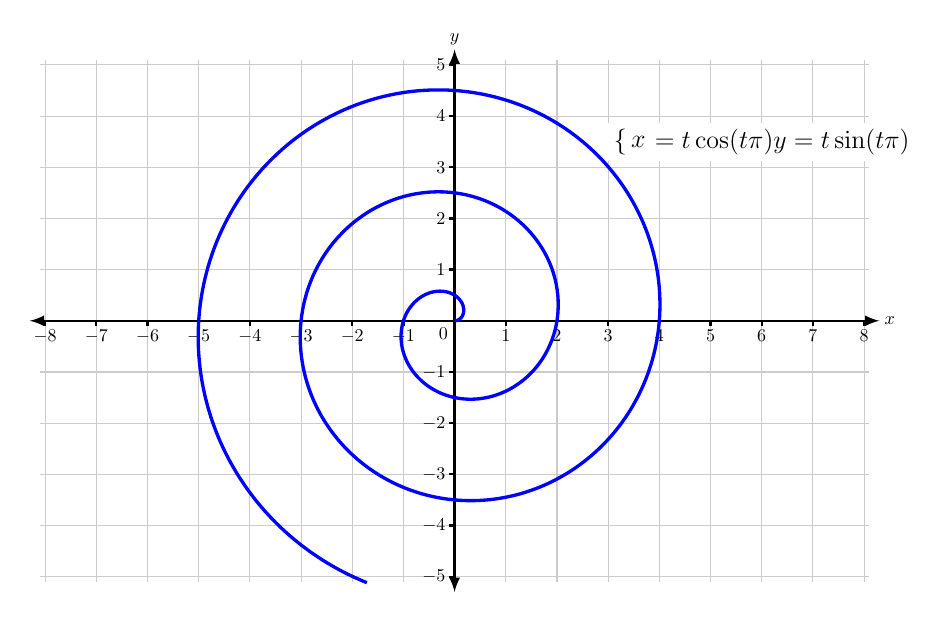
\begin{tikzpicture}[thick,scale=0.65, every node/.style={scale=0.65}]
  \def \minx {-8}
  \def \maxx {8}
  \def \miny {-5}
  \def \maxy {5}

  \draw[thin,black!20] (\minx-0.1,\miny-0.1) grid (\maxx+0.1,\maxy+0.1);

  \draw[thick, latex-latex] (\minx-0.3,0)--(\maxx+0.3,0);
  \draw[thick, latex-latex] (0,\miny-0.3)--(0,\maxy+0.3);
  \node at (\maxx+0.5,0) {$x$};
  \node at (0,\maxy+0.5) {$y$};

  \foreach \x in {\minx,...,-1}{
    \draw (\x,0)--(\x,-0.1);
    \node[below,black] at (\x,-0.05) {$\x$};
  }
  \foreach \x in {1,...,\maxx}{
    \draw (\x,0)--(\x,-0.1);
    \node[below,black] at (\x,-0.05) {$\x$};
  }
  \foreach \y in {\miny,...,-1}{
    \draw (0,\y)--(-0.1,\y);
    \node[left,black] at (-0.05,\y) {$\y$};
  }
  \foreach \y in {1,...,\maxy}{
    \draw (0,\y)--(-0.1,\y);
    \node[left,black] at (-0.05,\y) {$\y$};
  }
  \node[below left,black] at (0,0) {$0$};

  \draw[
    very thick,
    domain=0:5.4,
    variable=\t,
    smooth,
    samples=300,
    blue]
    plot ({\t*cos(\t*3.1415 r)},{\t*sin(\t*3.1415 r)});

  \node at (6,3.5) [fill=white]
  {
      \Large
      $
      \begin{cases}
        x = t \cos(t\pi) \\
        y = t \sin(t\pi)
      \end{cases}
      $
  };
\end{tikzpicture}

\end{frame}

%------------------------------------------------------------------------------%
\addtocounter{exemplo}{1}
\begin{frame}{Exemplo \theexemplo}
  A posição de uma partícula se movendo no plano $xy$ é dada por
  \[
    x = \sqrt{t}  \qquad
    y = t         \qquad
    t \geq 0
  \]

  Esboce sua trajetória
\end{frame}

%------------------------------------------------------------------------------%
\begin{frame}{Exemplo \theexemplo}
\begin{columns}
\column{0.4\linewidth}
  Eliminando $t$ em
  \begin{align*}
    x & = \sqrt{t} \\
    y & = t
  \end{align*}
  temos
  \[
    x
    = \sqrt{t}
    = \sqrt{y}
  \]

\column{0.4\linewidth}
  Elevando os dois lados ao quadrado
  \begin{align*}
    x   & = \sqrt{y}                \\
    x^2 & = \left(\sqrt{y}\right)^2
          = \abs{y}
          = y                       \\
    y   & = x^2
  \end{align*}
\end{columns}
\end{frame}

%------------------------------------------------------------------------------%
\framedgraphic{Exemplo \theexemplo}{exemplo_curvas_4}{}

%------------------------------------------------------------------------------%
\addtocounter{exemplo}{1}
\begin{frame}{Exemplo \theexemplo}
  Construa uma curva paramétrica cuja trajetória seja uma circunferência\\
  de raio 2 centrada em $(3, 4)$
\end{frame}

%------------------------------------------------------------------------------%
\begin{frame}{Exemplo \theexemplo}
\begin{columns}
\column{0.3\linewidth}
  Sabemos que
  \begin{align*}
    x & = \cos(t) \\
    y & = \sin(t) \\
    0 & \leq t < 2\pi
  \end{align*}
  parametriza uma circunferência de raio 1 centrada em \((0, 0)\)
\column{0.3\linewidth}
  \pause
  Para que o raio seja 2 multiplicamos as funções por 2
  \begin{align*}
    x & = 2\cos(t) \\
    y & = 2\sin(t) \\
    0 & \leq t < 2\pi
  \end{align*}
\column{0.3\linewidth}
  \pause
  Para mover o centro para $(3, 4)$ somamos esses valores
  \begin{align*}
    x & = 2\cos(t) + 3\\
    y & = 2\sin(t) + 4\\
    0 & \leq t < 2\pi
  \end{align*}
\end{columns}
\end{frame}

%------------------------------------------------------------------------------%
\section{Lista Mínima}

%------------------------------------------------------------------------------%
\begin{frame}{Lista Mínima}
  Cálculo Vol. 2 do Thomas 12\textsuperscript{a} ed. -- Seção 11.1
  \begin{enumerate}
    \item Estudar todo o texto da seção
    \item Resolver os exercícios: 3, 5, 11, 19, 21, 23, 31
  \end{enumerate}

  \vfill
  Atenção: A prova é baseada no livro, não nas apresentações
\end{frame}

%------------------------------------------------------------------------------%
\end{document}
%------------------------------------------------------------------------------%
